%%%% CLASS
% >
\documentclass[a4paper,twoside, openright,%draft
]{book}

\usepackage{titlesec}

% >\documentclass[10pt,a4paper,twoside,landscape,twocolumn]{book}
% >\documentclass[a4paper,twoside,draft]{book}%debug%

% >
\RequirePackage{JMR.old}%%

% >
\RequirePackage{UGE/UGE-Template}%%

% >
\RequirePackage{UGE/UGE-Thesis}%%

%% Compilation séparée
%\includeonly{src/Corps/Chap-1-Cadre-theorique}
%\includeonly{src/Corps/Chap-2-Revue-systematique}
%\includeonly{src/Corps/Chap-3-Methodologie}
%\includeonly{src/Corps/Chap-4-Profil-voyageurs}
%\includeonly{src/Corps/Chap-5-Distances-detours}
%\includeonly{src/Corps/Chap-6-Modelisation-NPART}
%\includeonly{src/Corps/0-Annexes}
%\includeonly{src/Corps/Donnees-ouvertes}

\usepackage{main-local}

\begin{document}

\setlist[itemize]{noitemsep} % Supprime les espacements entre les points

\graphicspath{%
  {./src/Figures/},{./UGE/},{./UGE/Logo/}
}

    % Page de garde
    \AddToShipoutPictureBG*{%
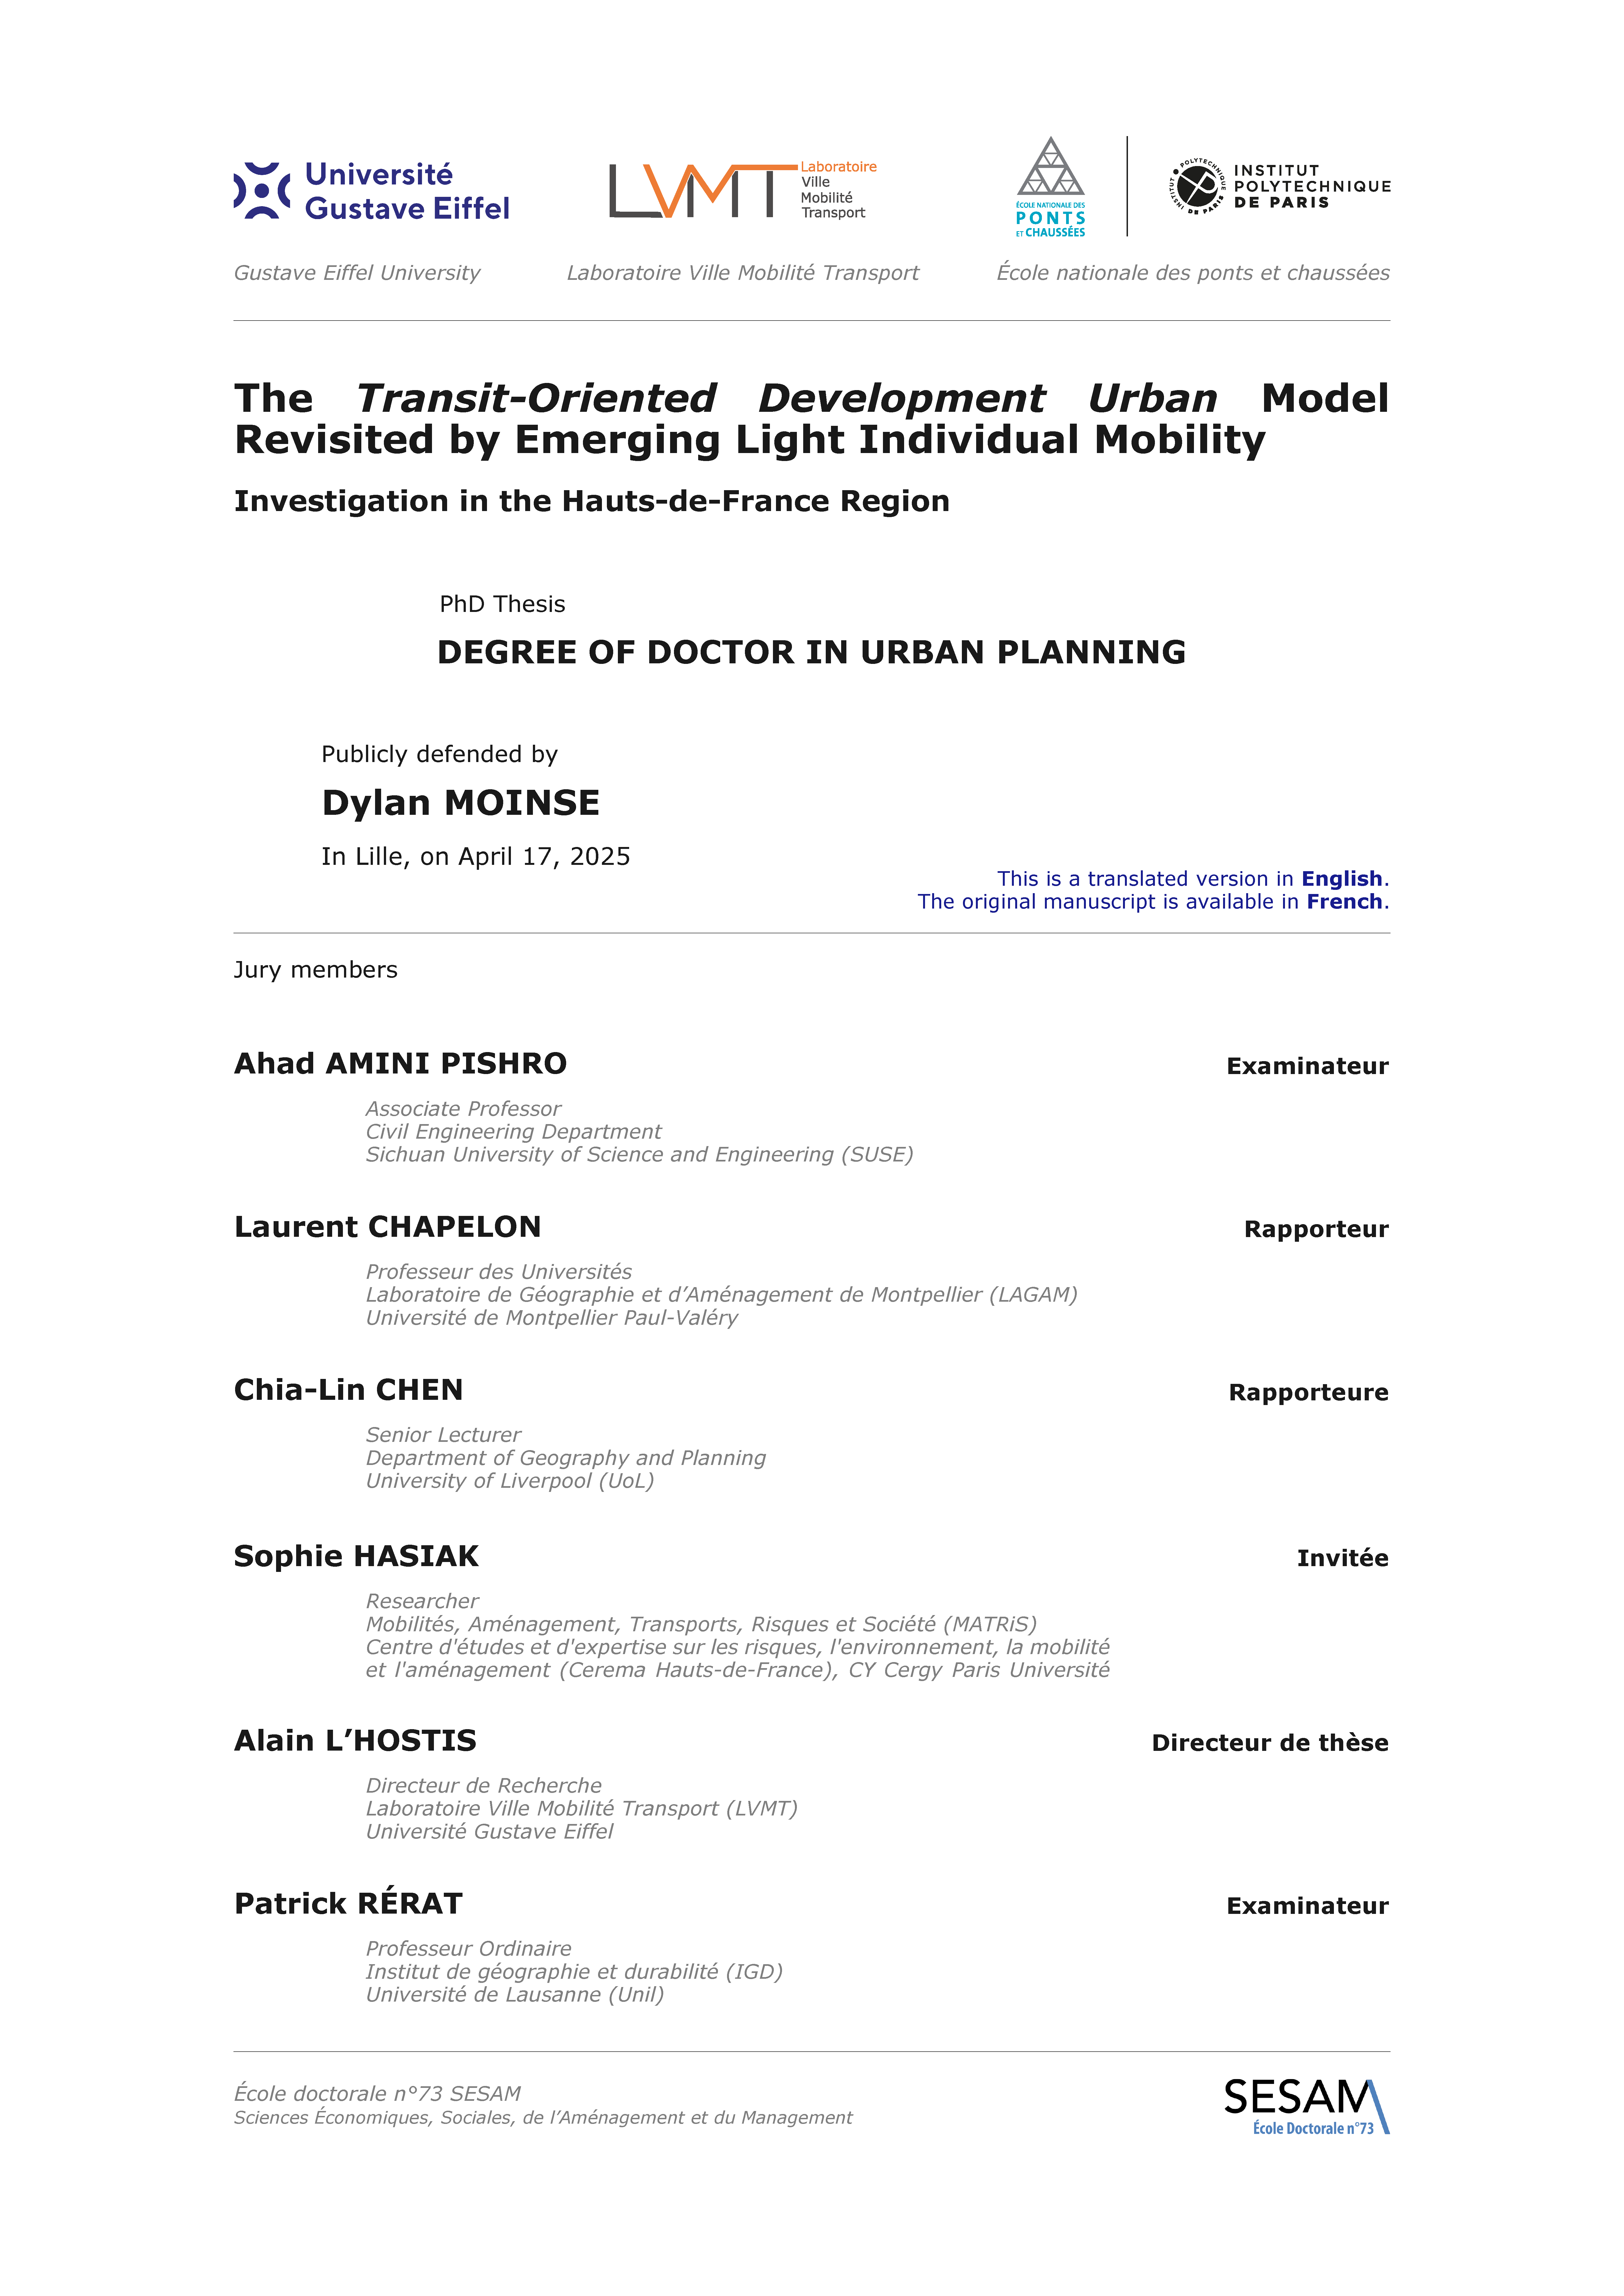
\includegraphics[width=\paperwidth,height=\paperheight]{src/Figures/Arriere_plan/EN_Page_de_garde.pdf}
    }
%\maketitle{}

\newpage
\null
\thispagestyle{empty}
\newpage
\thispagestyle{empty}

\pagestyle{UGEfancy} % À terme, renommer simplement en fancy

\cleardoublepage
\pagenumbering{Roman}
\setcounter{page}{1} % Commencer la numérotation à 1

%% ______________________________ %%
% BODY
\subfile{body}

\end{document}